\section{Pushbroom Hyperspectral Imager} \label{sec:hsi}
\begin{figure*}[htbp]
  \centering
      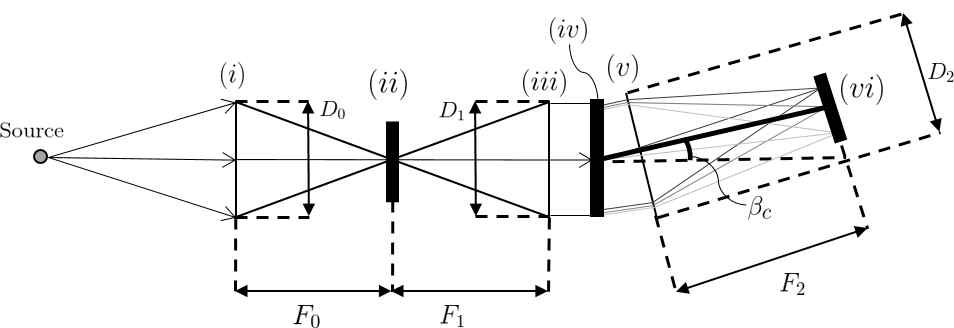
\includegraphics[width=0.7\textwidth]{figs/optics.png}
  \caption{Optical diagram of the pushbroom hyperspectral imager based on \cite{Sigernes18}.}
	\label{fig:optics}
\end{figure*}
% \textcolor{blue}{Contribution (2): "We present a COTS-assembled hyperspectral imager with high spectral resolution and efficiency designed for the HYPSO-1 mission and is based on \cite{Sigernes18}. We present the chosen components for the design that satisfy objectives of observing algal blooms, and show how SNR may be increased by binning operations." Key points to keep in mind while writing this section:
% \begin{itemize}
%     \item How does the proposed HSI work?
%     \item How is it performing from space on HYPSO-1?
% \end{itemize}}
\subsection{Optics}\label{sec:optics}
Emerging commercial off the shelf (COTS) products that are smaller in size make hyperspectral imaging accessible, flexible and affordable \cite{Sigernes18}. Such low-cost pushbroom cameras may in principle be designed and integrated into small-satellites.
\begin{figure}[htbp]
  \centering
      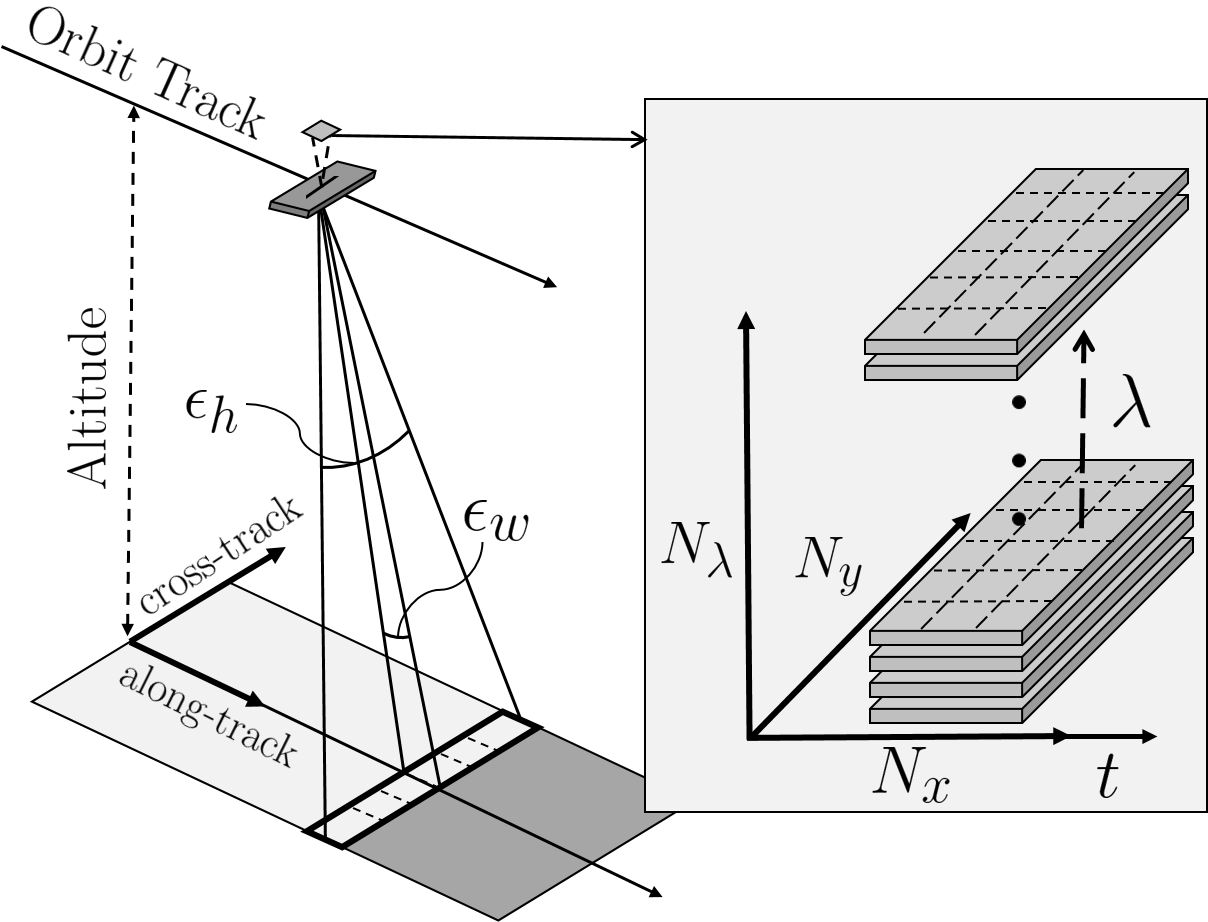
\includegraphics[width=0.45\textwidth]{figs/pushbroom_scanning.png}
  \caption{Data acquisition with pushbroom hyperspectral imaging.}
	\label{fig:push_scan}
\end{figure}
% Figure \ref{fig:push_scan} shows a satellite-based pushbroom hyperspectral imager collecting lines of cross-track pixels and spectral information, eventually forming a datacube. 
Figure \ref{fig:optics} shows the optical diagram of a center cross-section of the instrument parallel to the refraction axis. The components are: (i) front lens with aperture diameter $D_0$ and focal length $F_0$; (ii) entrance slit with dimensions $w_{\text{slit}}$ and $h_{\text{slit}}$ that are slit width and height, respectively; (iii) collimator lens with aperture diameter $D_1$ and focal length $F_1$; (iv) grating that receives the incoming light at angle $\alpha=0^{\circ}$ and diffracts the light at angle $\beta$ measured from the grating normal; and (v) detector lens with aperture diameter $D_2$ and focal length $F_2$. Finally, (vi) is the detector. The horizontal and vertical components of the FoV, $\epsilon_w \times \epsilon_h$, are found from the slit width and height as
\begin{subequations}
\begin{align}
\tan{\left(\frac{\epsilon_{w}}{2}\right)} &= \frac{w_{\text{slit}}}{2F_0}, \label{eq:fov_x} \\
\tan{\left(\frac{\epsilon_{h}}{2}\right)} &= \frac{h_{\text{slit}}}{2F_0}. \label{eq:fov_y}
\end{align} 
\end{subequations}

Assuming no loss of light transmission within the spectrometer from the front to the exit plane, the etendue is expressed as
\begin{equation}
G = \pi \frac{D_0^2}{4 F_0^2}\cos(\beta_c) w_{d} h_{d},
\end{equation}
\noindent where
\begin{subequations}
\begin{align}
h_{d} &= h_{\text{slit}}\frac{F_2}{F_1}, \label{eq:effective_height}\\
w_{d} &= \frac{w_{\text{slit}}F_2}{\cos(\beta_c)F_1} \label{eq:effective_width},
\end{align}
\end{subequations}
\noindent and $\beta_c$ is the diffraction angle at center wavelength $\lambda_c$ \cite{Lerner2006}. It is assumed that $\beta_c\approx\beta(\lambda)$ for all $\lambda$.
% The horizontal and vertical magnification of entrance slit image

The bandpass $BP$ for the optical system, or the recorded Full Width at Half Maximum (FWHM) of a monochromatic spectral
line, and is a measure of the instruments ability to separate adjacent spectral lines in the
spectrogram. Assuming no degradation due to aberrations and diffraction effects, the optical bandpass may be approximated as
\begin{align}
BP &\approx\frac{g w_{\text{slit}}}{\kappa F_1}, \label{eq:bp}
\end{align}
\noindent where $g$ is the grating groove spacing and $\kappa$ is the spectral order \cite{Lerner2006}. 
% For an emission with finite spectral bandwidth such as fluorescent light, in real-life the bandpass is also a function of the natural spectral bandwidth of the emitting source and the limiting resolution of the instrument, where the latter usually has a minuscule effect.
\subsection{Detector}
 $N_x$ lines with $N_y$ and $N_\lambda$ pixels each are collected sequentially during each camera integration time $\Delta t$, to form a threedimensional datacube. $N_y$ is the total number of spatial pixels perpendicular to the scan direction and $N_{\lambda}$ is the total number of pixels along the spectral dimension, cf. Figure \ref{fig:push_scan}. It is assumed that $\Delta t=1/FPS=\tau +\delta t$ is the associated camera integration time where $FPS$ is the frame rate, $\tau$ is the camera exposure time and $\delta t$ is the camera read-out time.
\begin{figure}[htbp]
  \centering
      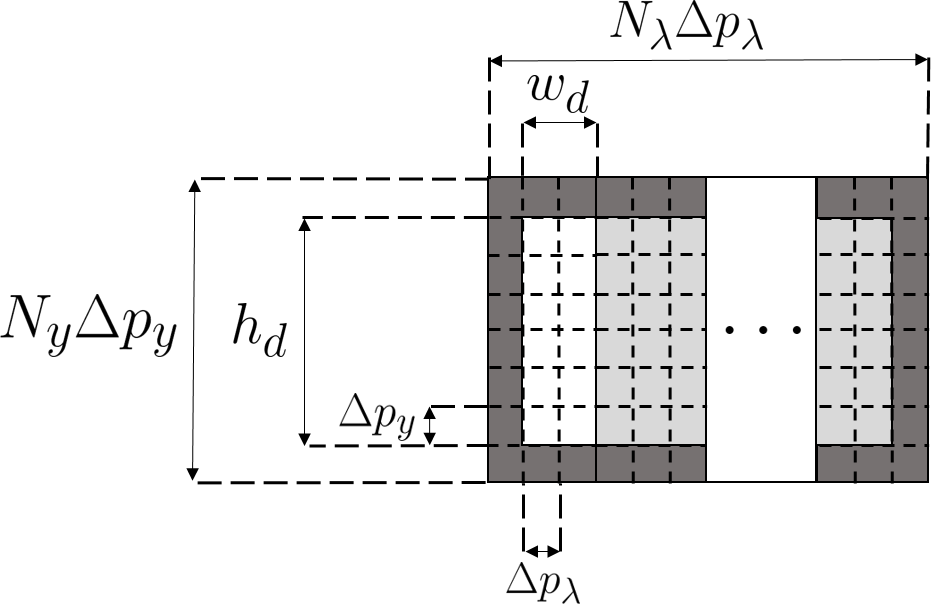
\includegraphics[width=0.4\textwidth]{figs/fad.png}
  \caption{Detector plane with $h_d$ and $w_d$ being the vertical and horizontal magnification of the entrance slit image. The camera's mechanical layout may block some of the light as shown by the darkest gray regions.}
	\label{fig:fad2}
\end{figure}
The rounded up amount of illuminated pixels in per magnified slit image, as shown in Figure \ref{fig:fad2}, are approximately
\begin{subequations}
\begin{align}
    N_{h} = \frac{h_d}{\Delta p_y}, \\
    N_{w} = \frac{w_d}{\Delta p_\lambda},
\end{align}
\end{subequations}
\noindent where $\Delta p_\lambda$ and $\Delta p_y$ are the width and height of a pixel, respectively.

With the ability to bin pixels, photon-electrons are gathered from adjacent pixels to create one merged pixel with higher SNR at the cost of reduced spectral or spatial resolution. The signal increases proportionally with the square root of number of binning operations $B_{\lambda}$ in the spectral direction or $B_{y}$ in the vertical spatial direction. 
\subsection{Signal-to-Noise Ratio}
The photon flux into the detector may be written as
\begin{equation}
\dot{\Phi}(\lambda) = L(\lambda)\eta_0 \eta_1 \eta_{G}(\lambda) \eta_2 G \lambda\frac{ BP}{h_{\text{planck}}c}, \label{eq:photons}
\end{equation}
\noindent where $L(\lambda)$ is the radiance as a function of wavelength reaching the sensor, $\eta_0, \eta_1, \eta_2$ are the optical efficiencies of the front, collimator and detector lenses respectively, $\eta_G$ is the grating efficiency, $c$ is the speed of light, and $h_{\text{planck}}=6.62607015\times10^{-34}$ $\rm{Js}$ is the Planck constant. 

The number of photons converted to electrons in each pixel is
\begin{equation}
c_{\text{electrons}} = \frac{\eta_{\text{QE}}(\lambda)\dot{\Phi}(\lambda)\tau}{N_{w}N_{h}}, \label{eq:photons2}
\end{equation}
\noindent where $\eta_{\text{QE}}(\lambda)$ is the quantum efficiency of the detector. Assuming that $c_{\text{electrons}}$ has a Poisson probability distribution, then the SNR in one unbinned pixel is
\begin{align}
SNR_{[1, 1]} 
&=\frac{c_{\text{electrons}}}{\sqrt{c_{\text{electrons}} + c_{\text{dark}}+c_{\text{read-out}}^2+c_{\text{dig}}^2}}.  \label{eq:snr}
\end{align}
\noindent where $c_{\text{dark}}=i_{\text{dark}}\Delta t$ is represented with a Poisson probability distribution, while $c_{\text{read-out}}$ and $c_{\text{dig}}$ are assumed to have Gaussian probability distribution with zero mean \cite{Moses2012, Skauli2011}. $i_{\text{dark}}\Delta t$ is the average shot noise registered due to dark current $i_{\text{dark}}$, $c_{\text{read-out}}$ is the standard deviation of electrons due to the sensor read-out circuits, and $c_{\text{dig}}=c_{\text{electrons},\text{max}}/(2^{b}\sqrt{12})$ is the standard deviation of digitization (or quantization) noise where $c_{\text{electrons},\text{max}}$ is the well depth of electrons and $b$ is the Analog-to-Digital Converter (ADC) bit depth.

To match the optical bandpass then we must bin $B_\lambda=\ceil{N_w}$ pixels in the spectral direction where $\ceil{\cdot}$ means rounding up to an integer, rendering the SNR in a $[\ceil{N_w}, 1]$ window to be $SNR_{[\ceil{N_w}, 1]} \approx \sqrt{N_w}SNR_{[1,1]}$. Binning may also be applied for the spatial pixels. In particular, if large distances are covered during each camera exposure time such as for HYPSO-1, the partial overlap of frames in the along-track direction may be utilized to predict the benefits of super-resolution algorithms.

\subsection{Payload Design} \label{sec:payload-hsi}
HYPSO-1's payload, shown in Figure \ref{fig:HSI}, is built with mainly COTS products from Thorlabs and Edmund Optics and a few 3D-printed parts \cite{Sigernes18}. The design provides a spectral range in the visual and near-infrared part of the spectrum and bandpass of $3.33 \hspace{3pt} \rm{nm}$ which fulfills HYPSO-1 mission requirements to observe algal blooms and primary productivity. In theory, the f-numbers should be equal to maximize the light throughput in the optics, however these are set to $F_0/\#=F_1/\#=2.8$ and $F_2/\#=2$ to avoid stray light effects. The instrument's specifications and performance are given in Table \ref{tab:optics}.
\begin{figure}[tbhp]
  \begin{center}
    %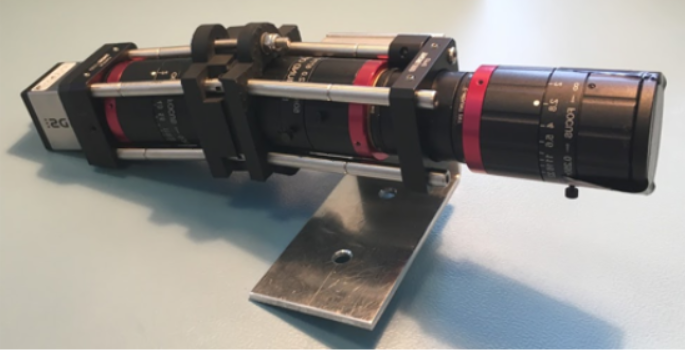
\includegraphics[width=70mm,angle=0]{figs/HSI_v6.PNG}
    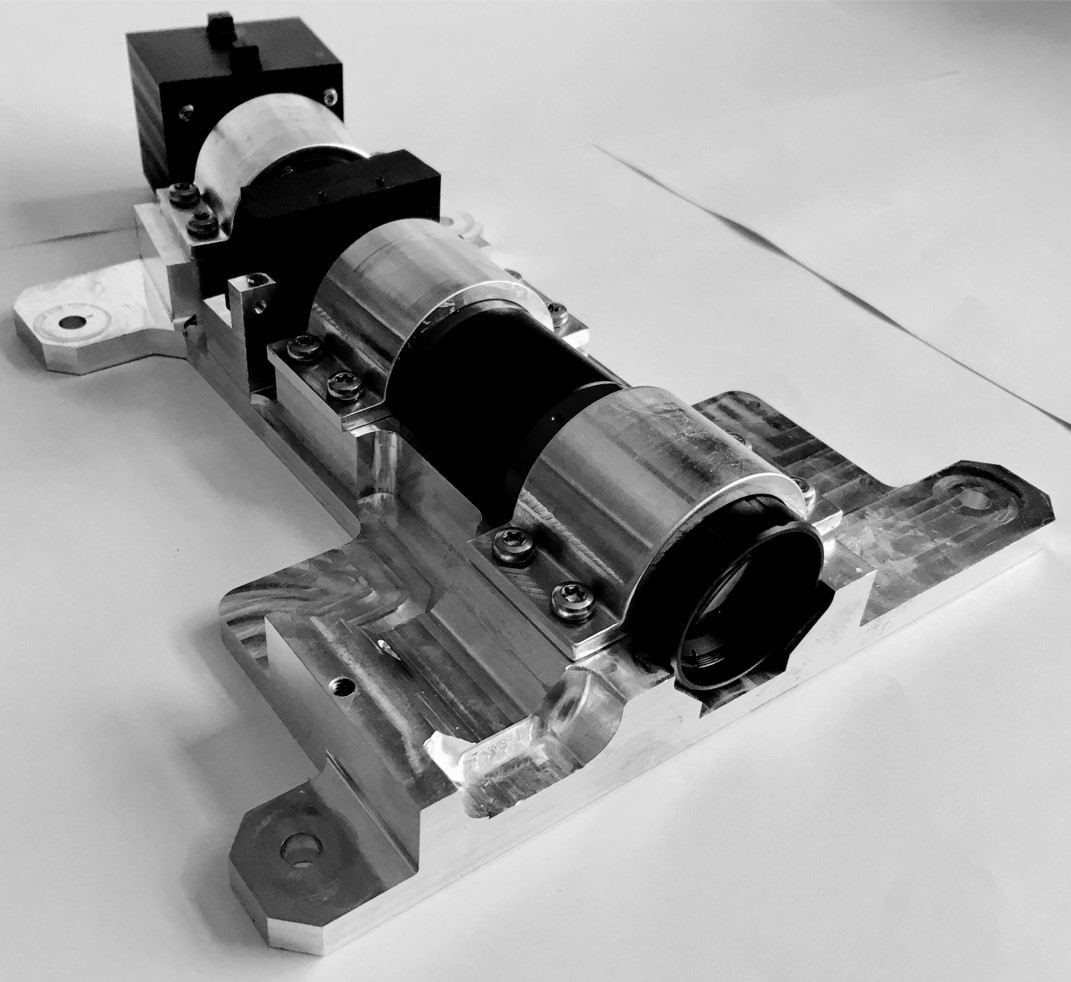
\includegraphics[width=60mm,angle=0]{figs/HSI.jpg}  %more options in figs/mech folder
    \caption{Hyperspectral imager payload assembled for CubeSat integration}
    \label{fig:HSI}
\end{center}
\end{figure}

The chosen sensor is the SONY IMX249 mounted in an industrial camera head from The Imaging Source Europe GmbH. It has a reported well depth of about 33022 $e^{-}$, equivalent to a maximum SNR of approximately $181.6$ or $45.2 \hspace{3pt} \rm{dB}$ per pixel if not binned.The detector enables a maximum frame rate of up to $FPS=47$, but due to constraints on the data throughput the practical FPS setting is governed by the number of binning operations, subsampling of pixels and the chosen window of pixels, commonly named as the Area of Interest (AoI).
\begin{table}[htbp]
	\caption{Hyperspectral imager specifications}
	\label{tab:optics}
	\centering
			\begin{tabular}{l l}
				\hline
				Parameter & Value \\
				\hline 
				FoV $\epsilon_w \times \epsilon_h$ &	$0.0564^{\circ} \times 7.8826^{\circ}$  \\
				$F_0=F_1=F_2$ & 50 $\hspace{3pt} \rm{mm}$ \\
				$F_0/\#=F_1/\#$ & 2.8  \\
				$F_2/\#$ & 2 \\
				$D_0=D_1$  & 17.9 $\hspace{3pt} \rm{mm}$ \\
				$D_2$ &  25 $\hspace{3pt} \rm{mm}$ \\
				Slit width $w_{\text{slit}}$ & 50 $\hspace{3pt} \mu\rm{m}$ \\
				Slit height $h_{\text{slit}}$ & 7 $\hspace{3pt} \rm{mm}$ \\
				Optical efficiency $\eta_{0}=\eta_{1}=\eta_{2}$ & $0.8$ \\
				Grating efficiency $\eta_{G}$ @$500\hspace{3pt} \rm{nm}$ & 0.73 \\
				Spectral order $\kappa$ & 1 \\
				Groove spacing $g$ & 3333.33 $\hspace{3pt} \rm{nm}$ \\
				Diffraction angle $\beta_c$ & 10.37$^{\circ}$ \\
				Pixel size $\Delta p_\lambda=\Delta p_y$ & $5.86 \hspace{3pt} \mu\rm{m}$ \\
				% Full detector resolution & $1936 \times 1216 \hspace{3pt} \rm{pixels}$ \\
				Usable detector resolution & $1936 \times 1194  \hspace{3pt} \rm{pixels}$ \\
				Quantum efficiency $\eta_{QE}$ @$500\hspace{3pt} \rm{nm}$ & 0.77 \\
				Spectral range &  $271-1006 \hspace{3pt} \rm{nm}$ \\ 
			    Bandpass $BP$ & $3.33 \hspace{3pt} \rm{nm}$ \\
				Dark current $i_{\text{dark}}$ & $0.95 \hspace{3pt} \rm{e}^{-}/\rm{s}$ \\
				Read-out noise $c_{\text{read-out}}$ & $6.93 \hspace{3pt} \rm{e}^{-}$ \\
				Quantization noise $c_{\text{dig}}$ & $2.33 \hspace{3pt} \rm{e}^{-}$ \\
				Max. SNR per pixel (unbinned) & $181.6$ ($45.2 \hspace{3pt} \rm{dB}$) \\
			    ADC bit-depth & $12\hspace{3pt}\rm{bits}$ \\
			 %   AoI & $1280 \times 720$ pixels \\
			 %  Binning $B_\lambda \times B_y$ & $6 \times 1$ \\
			 %  Subsampling & 2 \\
  		    % FPS $\zeta$ & Up to $47$ \\
				\hline
				\end{tabular}
\end{table}
% \begin{figure}[H]
%   \centering
%       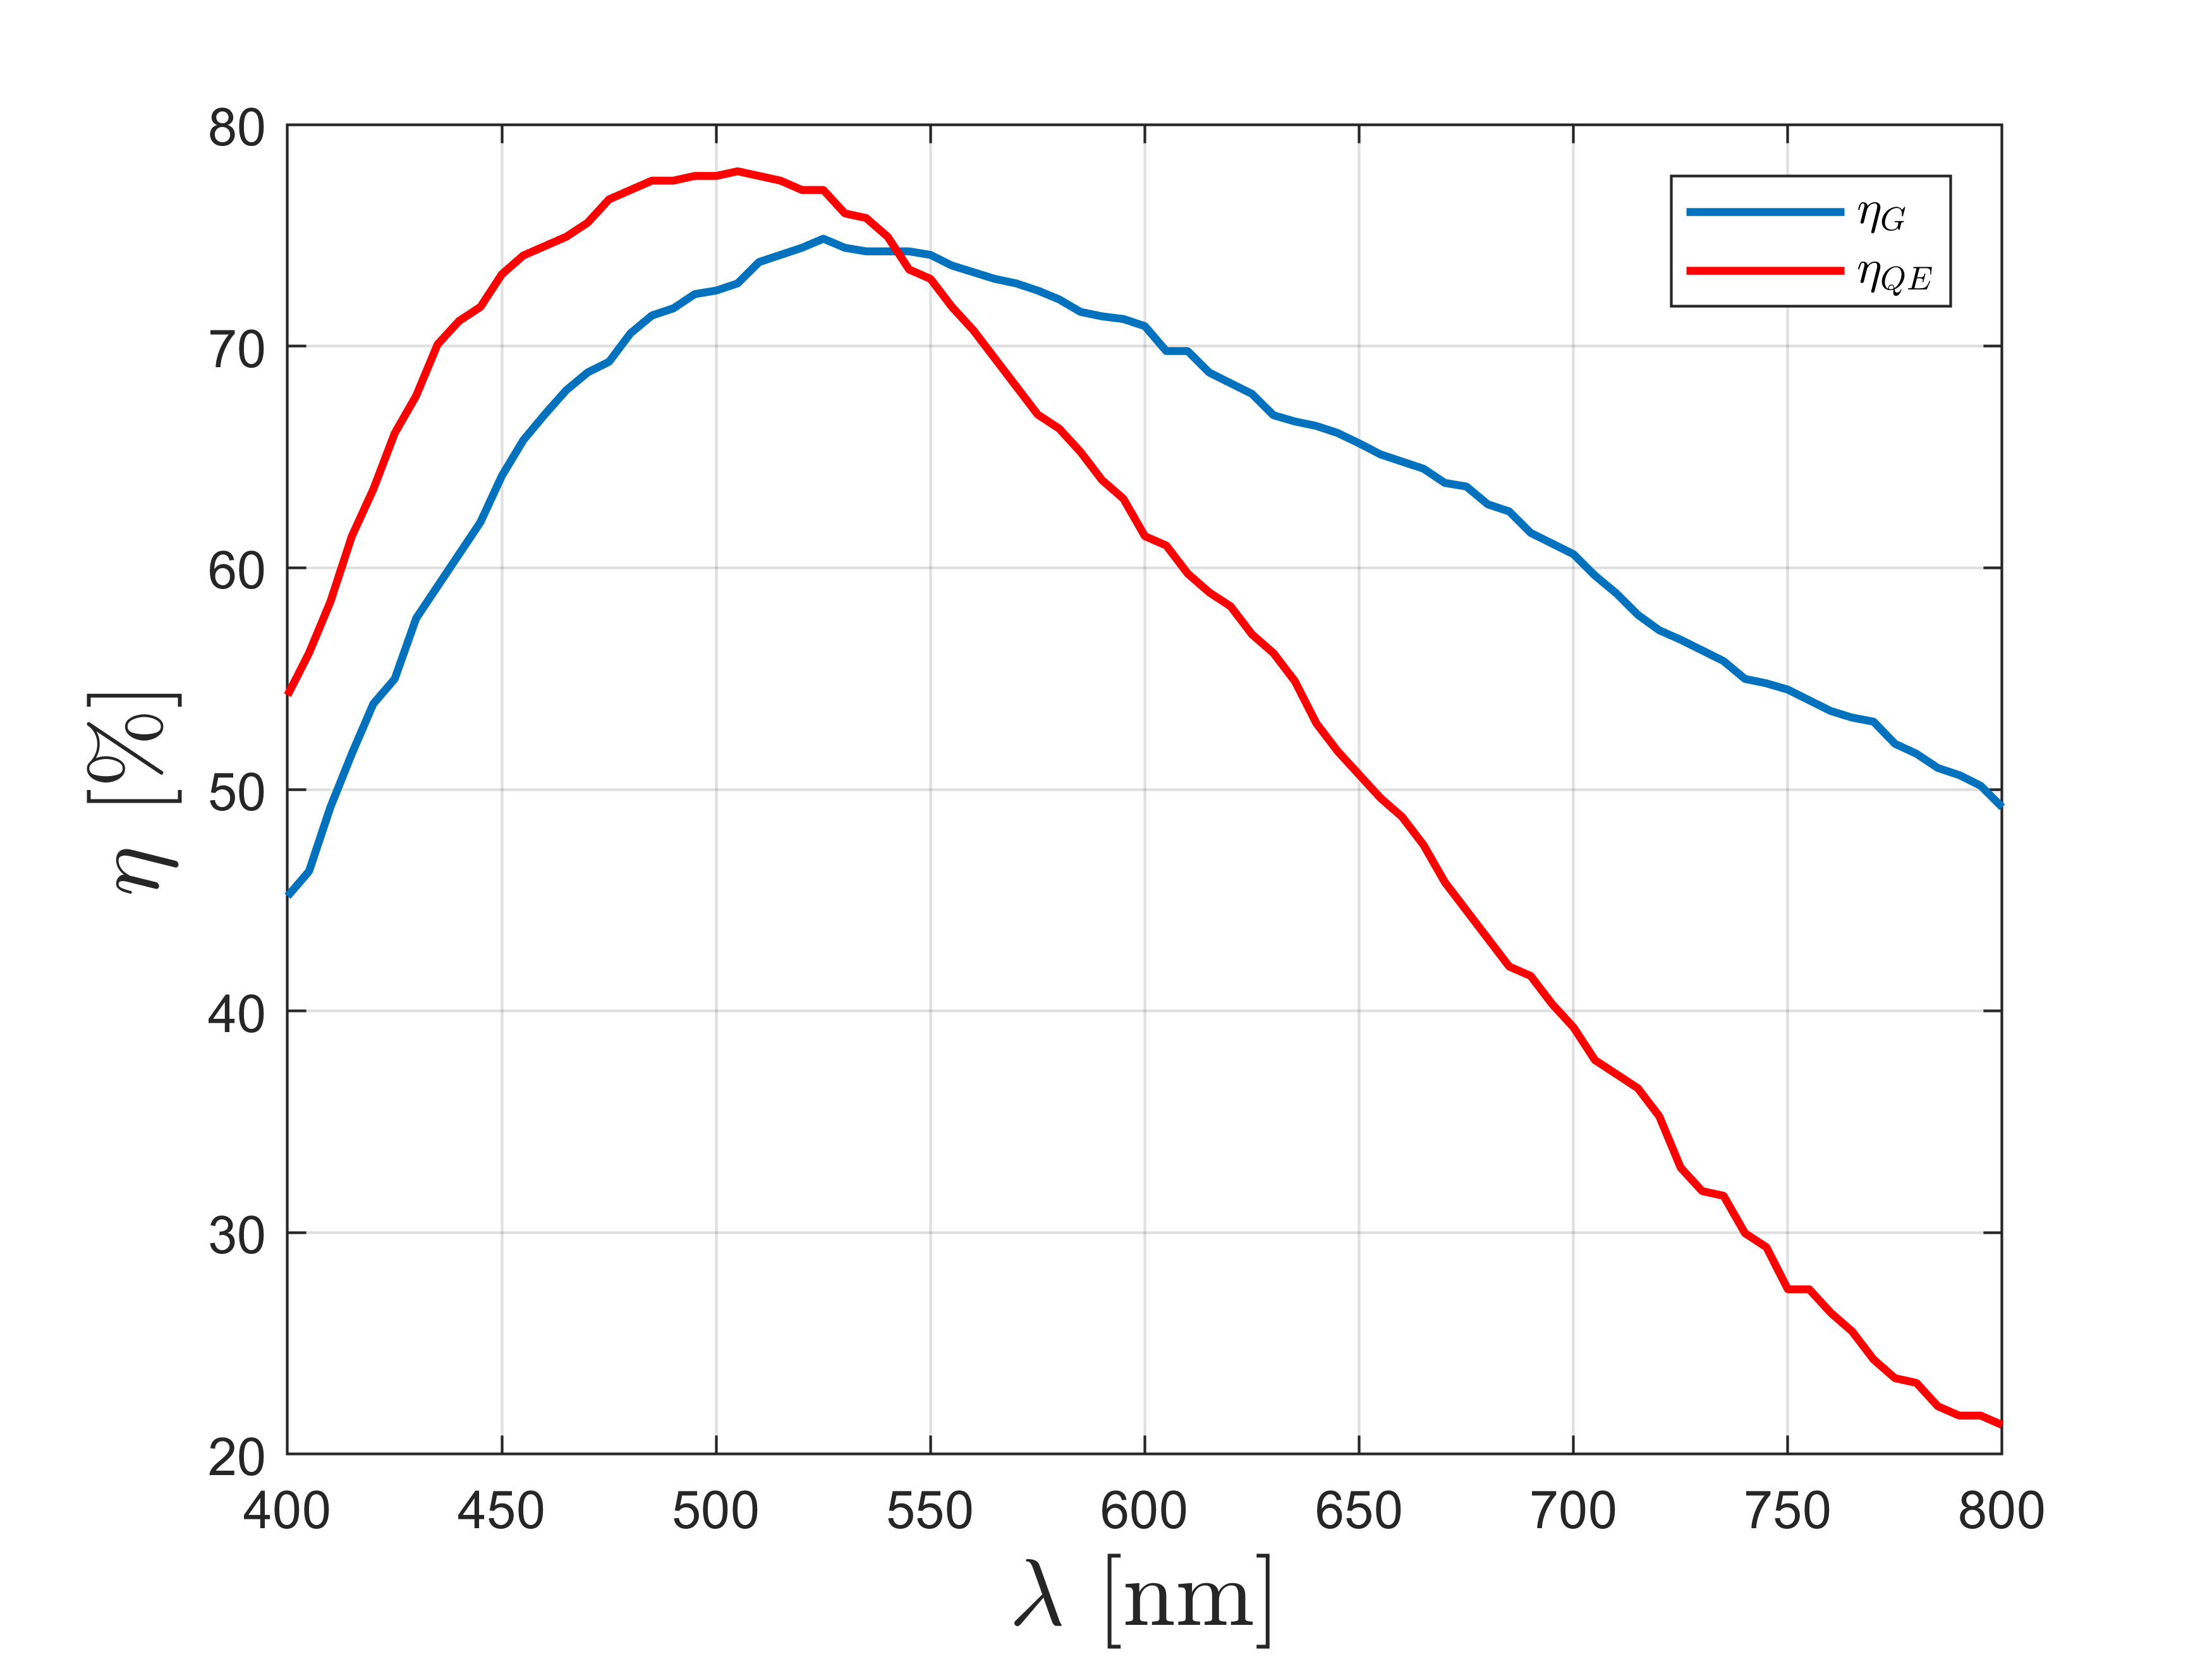
\includegraphics[width=0.45\textwidth]{figs/optical_eff.png}
%   \caption{Efficiencies for the grating and sensor SONY IMX249 across the spectral range.}
% 	\label{fig:optical_eff}
% \end{figure}